\documentclass[a4paper]{article}
\usepackage[top=0.5cm, bottom=0cm, left=0.5cm, right=0.5cm]{geometry}
\usepackage{tikz}
\usetikzlibrary{patterns}
\usetikzlibrary{shapes,arrows}
\usetikzlibrary{decorations.pathreplacing, positioning}

\begin{document}
\noindent
  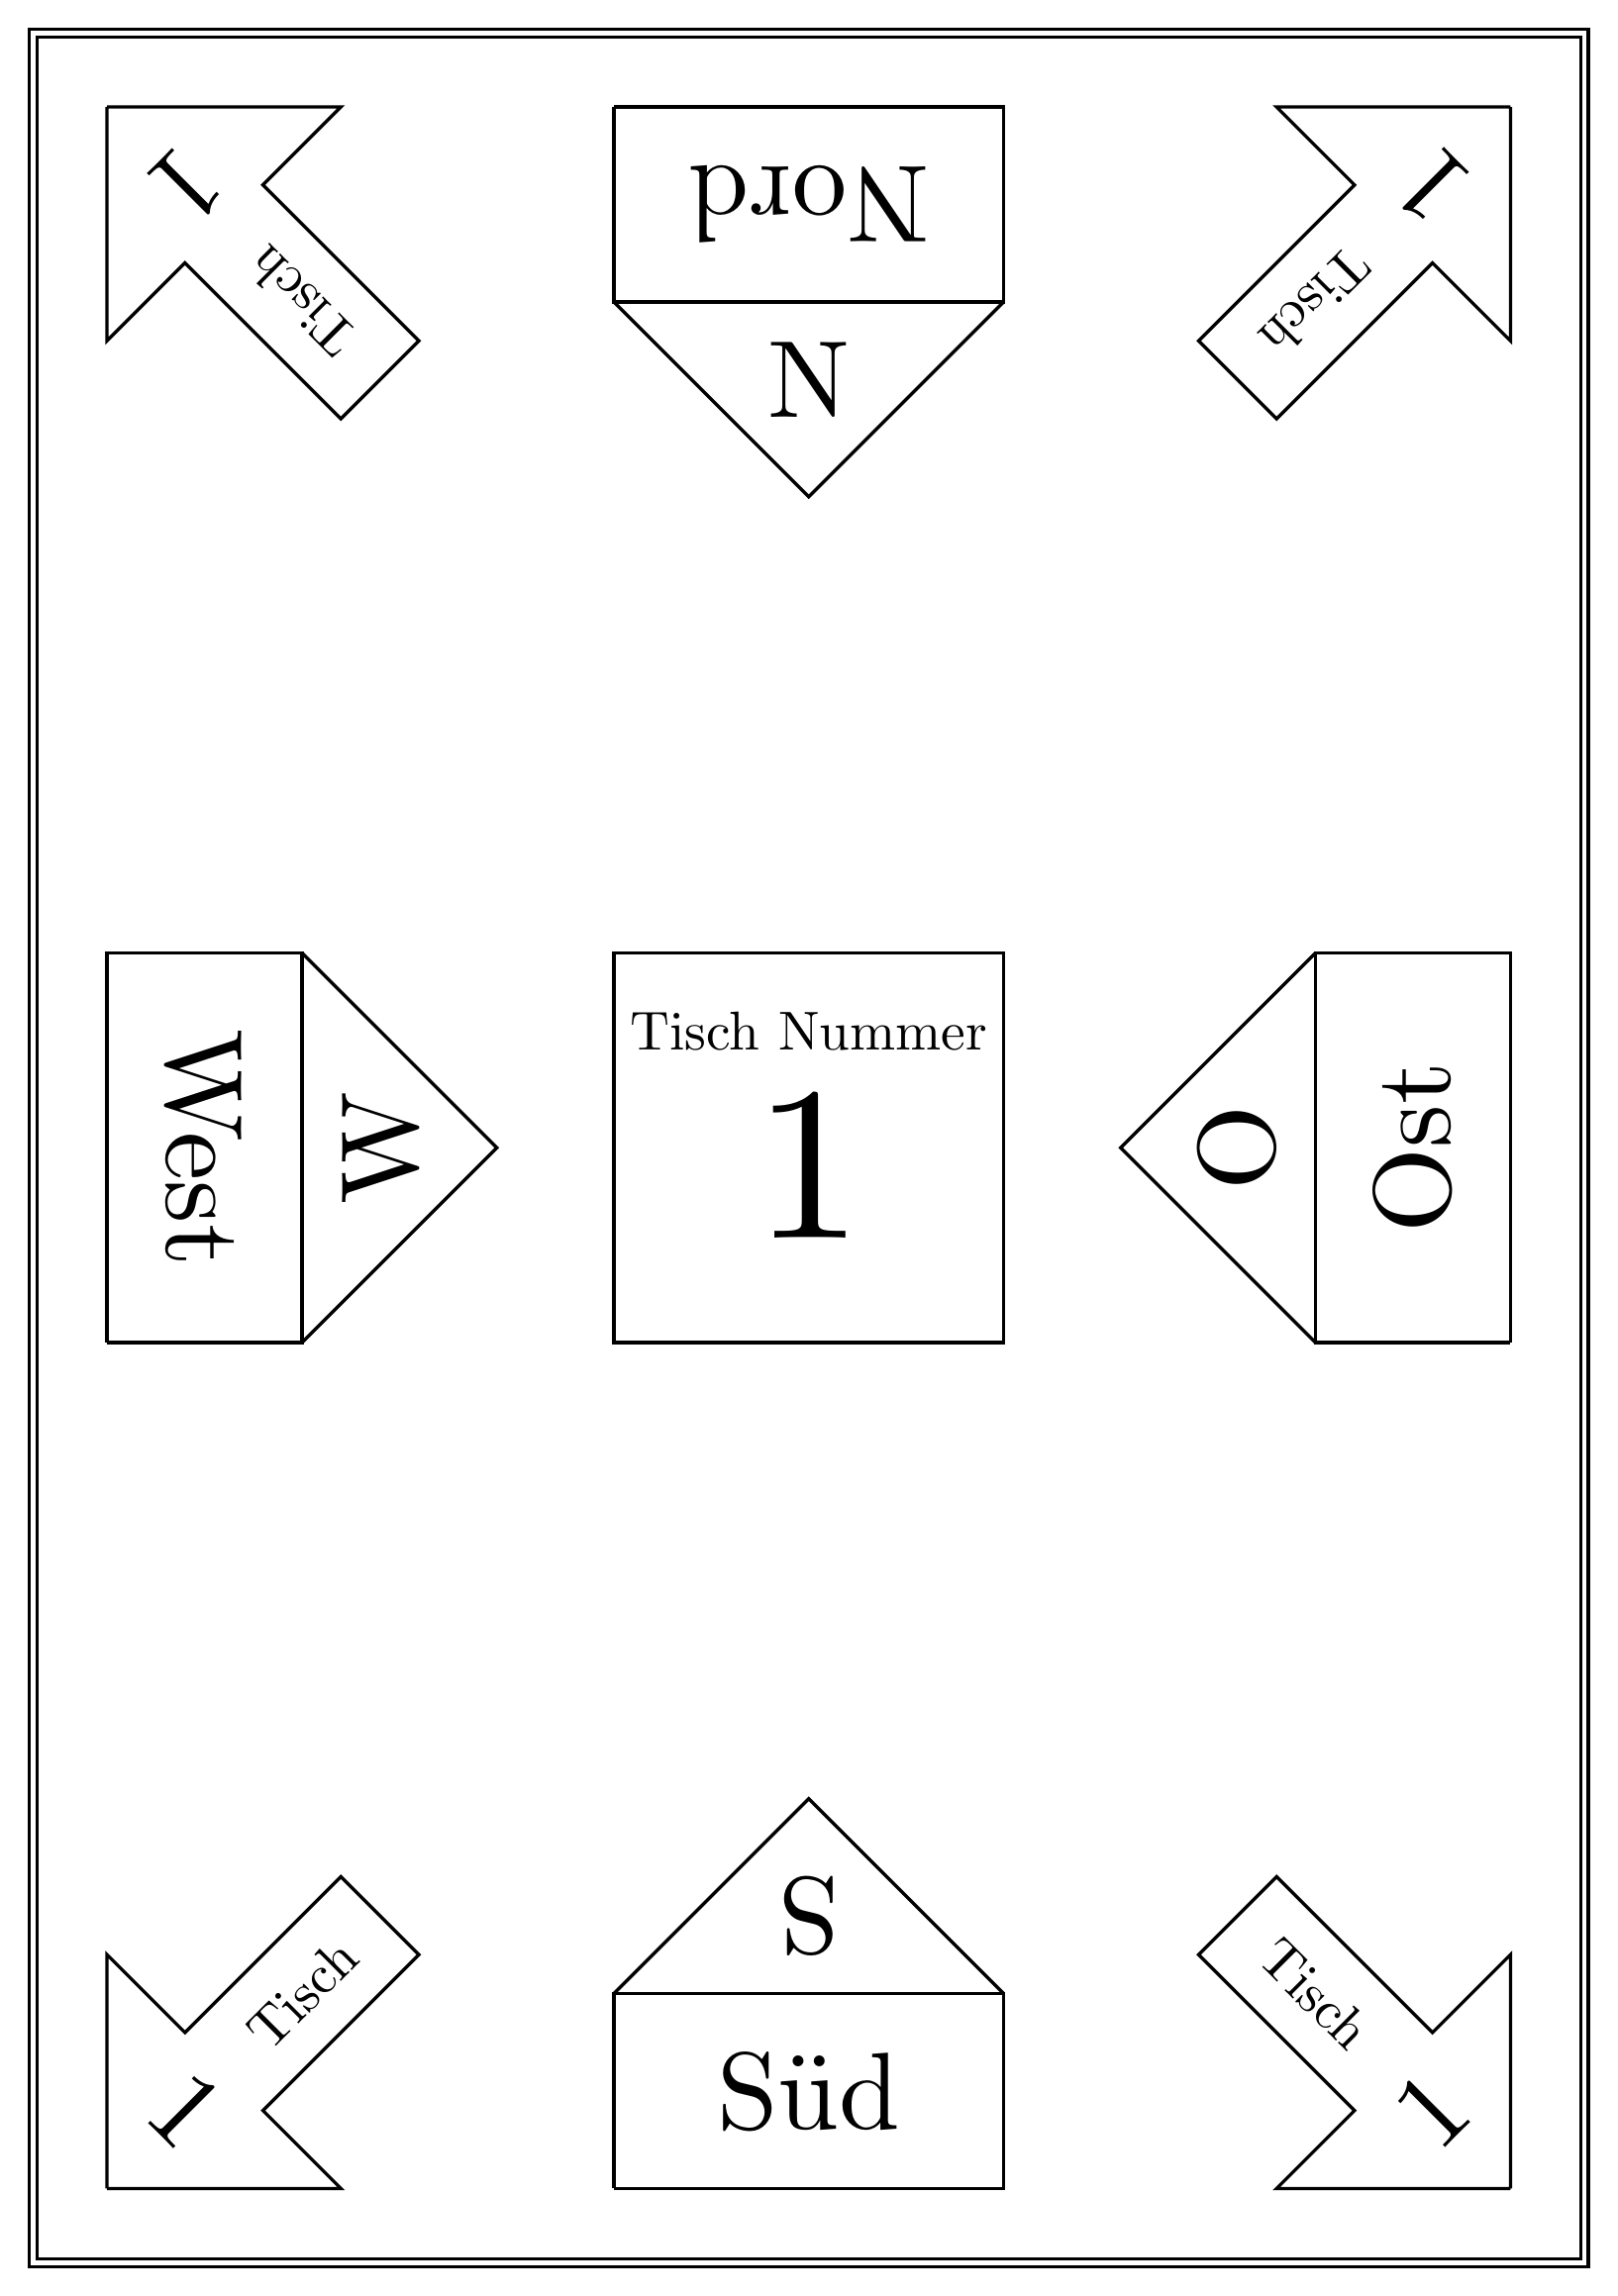
\begin{tikzpicture}

    % Border
    \draw[very thick] (0cm,0cm) rectangle (20.cm,28.7cm);
    \draw[very thick] (0.1cm,0.1cm) rectangle (19.9cm,28.6cm);

    % Table Nr
    \drawvery [thick] (7.4cm,11.75) rectangle (12.6cm,16.95cm);
    \draw[very thick] (7.5cm,11.85) rectangle (12.5cm,16.85cm);

    \node[very thick, scale=2] at (10cm, 15.85cm) {Tisch Nummer};
    \node[very thick, scale=8] at (10cm, 14.1cm) {1};

    % Arrows
    % SW
    \draw[very thick] (1cm, 1cm) -- (4cm, 1cm) -- (3cm, 2cm) -- (5cm, 4cm) -- (4cm, 5cm) -- (2cm, 3cm) -- (1cm, 4cm) -- (1cm, 1cm);
    \node[very thick, rotate=315, scale=4] at (2cm, 2cm) {1};
    \node[very thick, rotate=45, scale=2] at (3.5cm, 3.5cm) {Tisch};

    % SE
    \draw[very thick] (19cm, 1cm) -- (16cm, 1cm) -- (17cm, 2cm) -- (15cm, 4cm) -- (16cm, 5cm) -- (18cm, 3cm) -- (19cm, 4cm) -- (19cm, 1cm);
    \node[very thick, rotate=45, scale=4] at (18cm, 2cm) {1};
    \node[very thick, rotate=315, scale=2] at (16.5cm, 3.5cm) {Tisch};

    % NE
    \draw[very thick] (19cm, 27.7cm) -- (16cm, 27.7cm) -- (17cm, 26.7cm) -- (15cm, 24.7cm) -- (16cm, 23.7cm) -- (18cm, 25.7cm) -- (19cm, 24.7cm) -- (19cm, 27.7cm);
    \node[very thick, rotate=135, scale=4] at (18cm, 26.7cm) {1};
    \node[very thick, rotate=225, scale=2] at (16.5cm, 25.2cm) {Tisch};

    % NW
    \draw[very thick] (1cm, 27.7cm) -- (4cm, 27.7cm) -- (3cm, 26.7cm) -- (5cm, 24.7cm) -- (4cm, 23.7cm) -- (2cm, 25.7cm) -- (1cm, 24.7cm) -- (1cm, 27.7cm);
    \node[very thick, rotate=225, scale=4] at (2cm, 26.7cm) {1};
    \node[very thick, rotate=135, scale=2] at (3.5cm, 25.2cm) {Tisch};

    % Player Direction
    \draw[very thick] (7.5cm, 1cm) -- (7.5cm, 3.5cm) -- (12.5cm, 3.5cm) -- (12.5cm, 1cm) -- (7.5cm, 1cm);
    \draw[very thick] (7.5cm, 3.5cm) -- (10cm, 6cm) -- (12.5cm, 3.5cm);
    \node[very thick, scale = 4] at (10cm, 2.25cm) {Süd};
    \node[very thick, scale = 4, rotate=180] at (10cm, 4.5cm) {S};

    \draw[very thick] (7.5cm, 27.7cm) -- (7.5cm, 25.2cm) -- (12.5cm, 25.2cm) -- (12.5cm, 27.7cm) -- (7.5cm, 27.7cm);
    \draw[very thick] (7.5cm, 25.2cm) -- (10cm, 22.7cm) -- (12.5cm, 25.2cm);
    \node[very thick, scale = 4, rotate=180] at (10cm, 26.45cm) {Nord};
    \node[very thick, scale = 4] at (10cm, 24.2cm) {N};

    \draw[very thick] (1cm, 11.85) -- (1cm, 16.85cm) -- (3.5cm, 16.85cm) -- (3.5cm, 11.85cm) -- (1cm, 11.85cm);
    \draw[very thick] (3.5cm, 16.85cm) -- (6cm, 14.35cm) -- (3.5cm, 11.85cm);
    \node[very thick, scale = 4, rotate=270] at (2.25cm, 14.35cm) {West};
    \node[very thick, scale = 4, rotate=90] at (4.5cm, 14.35cm) {W};

    \draw[very thick] (19cm, 11.85) -- (19cm, 16.85cm) -- (16.5cm, 16.85cm) -- (16.5cm, 11.85cm) -- (19cm, 11.85cm);
    \draw[very thick] (16.5cm, 16.85cm) -- (14cm, 14.35cm) -- (16.5cm, 11.85cm);
    \node[very thick, scale = 4, rotate=90] at (17.75cm, 14.35cm) {Ost};
    \node[very thick, scale = 4, rotate=270] at (15.5cm, 14.35cm) {O};

    \end{tikzpicture}%
\end{document}
